% ------------------------------------------------------------------------
% bjourdoc.tex for birkjour.cls*******************************************
% ------------------------------------------------------------------------
%%%%%%%%%%%%%%%%%%%%%%%%%%%%%%%%%%%%%%%%%%%%%%%%%%%%%%%%%%%%%%%%%%%%%%%%%%

\documentclass{birkjour}
%
%
% THEOREM Environments (Examples)-----------------------------------------
%
 \newtheorem{thm}{Theorem}[section]
% \newtheorem{cor}[thm]{Corollary}
% \newtheorem{lem}[thm]{Lemma}
% \newtheorem{prop}[thm]{Proposition}
% \theoremstyle{definition}
 \newtheorem{defn}[thm]{Definition}
% \theoremstyle{remark}
% \newtheorem{rem}[thm]{Remark}
% \newtheorem*{ex}{Example}
 \numberwithin{equation}{section}

\usepackage[noadjust]{cite}
\usepackage{amsfonts}
\usepackage{listings}
\usepackage{algorithm}
\usepackage{algorithmic}
\usepackage{booktabs}
\usepackage{float}
\usepackage{caption}

\begin{document}

%-------------------------------------------------------------------------
% editorial commands: to be inserted by the editorial office
%
%\firstpage{1} \volume{228} \Copyrightyear{2004} \DOI{003-0001}
%
%
%\seriesextra{Just an add-on}
%\seriesextraline{This is the Concrete Title of this Book\br H.E. R and S.T.C. W, Eds.}
%
% for journals:
%
%\firstpage{1}
%\issuenumber{1}
%\Volumeandyear{1 (2004)}
%\Copyrightyear{2004}
%\DOI{003-xxxx-y}
%\Signet
%\commby{inhouse}
%\submitted{March 14, 2003}
%\received{March 16, 2000}
%\revised{June 1, 2000}
%\accepted{July 22, 2000}
%
%
%
%---------------------------------------------------------------------------
%Insert here the title, affiliations and abstract:
%


\title[A Fast Rotation Estimator in Geometric Algebra]
 {A Fast Rotation Estimator in Geometric Algebra}

%----------Author 1
\author[Mauricio Cele Lopez Belon]{Mauricio Cele Lopez Belon}
\address{Buenos Aires, Argentina}
\email{mclopez@outlook.com}

%\thanks{This work was completed with the support of our \TeX-pert.}
%----------Author 2
\author[Jin Wu]{Jin Wu}
\address{University of Electronic Science and Technology of China, Chengdu, China}
\email{jin\_wu\_uestc@hotmail.com}

%----------classification, keywords, date
\subjclass{Parallel algorithms 68W10; Clifford algebras, spinors 15A66}

\keywords{Geometric Algebra, Rotation Estimation, Wahba Problem}

\date{October 31, 2016}
%----------additions
%\dedicatory{To my wife}
%%% ----------------------------------------------------------------------

\begin{abstract}

We present a fast estimator of the best rotation aligning two sets of corresponding vectors (also known as Wahba's problem). The proposed method is among the fastest methods reported in literature, moreover it is robust to noise, accurate and simpler than most other methods. It is based on solving the linear equations derived from the formulation of the problem in Geometric Algebra.

\end{abstract}

%%% ----------------------------------------------------------------------
\maketitle
%%% ----------------------------------------------------------------------
%\tableofcontents
\section{Introduction}

\indent Wahba's problem has been studied for over half a century since 1965 \cite{Wahba1965}. The problem seeks the optimal rotation between two sets of corresponding vectors. Until now, some effective algorithms have been proposed to solve the problem, including QUEST, Euler-q and FLAE \cite{Mortari1996,Shuster1981,Wu2017,Yang2015}. Not only for aerospace engineering computation of spacecraft attitude, the Wahba's solutions are applied to the mesh deformation in computer graphics \cite{Sorkine2007, Sin2013} for accurate motion construction and restoration \cite{Nieto2012,Perwass2009}. For computer engineering, the accuracy requirements are not so high as that in aerospace engineering. As mentioned in \cite{Wu2017}, the solving accuracy for non-extreme data sets can reach to the level of $1\times10^{-14}$ for accurate navigation. For normal storage of floating numbers in nowadays computers, the accuracy is only about $1\times10^{-6}$ to $1\times10^{-8}$, owning far less required word-length than aerospace ones. By swapping the accuracy with computation time, in this paper, we solve the problem of estimating the best rotation for the alignment of two sets of corresponding vectors (also known as Wahba's problem). The proposed method is fast, robust to noise, accurate and simple. It is based on solving the linear equations derived from the formulation of the problem in geometric algebra.

Few work has been done on studying this problem using geometric algebra. Geometric algebra rotors are closely related to quaternions (quaternion algebra can be regarded as a geometric algebra defined on a set of imaginary basis vectors) we find geometric algebra to be a more natural choice for studying this problem since it is defined over a Euclidean vector space $\mathbb R^3$, where original data is defined. Given the prevalence of quaternions in literature it is somewhat surprising that a similar solution in quaternion form has never been discovered, it seem that such solution was waiting for the appearance of geometric algebra. The implementation of our algorithm does not require access to any geometric algebra library, we present an implementation based on standard matrix and quaternion library. 

\indent This paper is arranged as follows: Section II introduces the geometric algebra $\mathbb{G}_3$, Section III includes the presentation of our fast rotor estimation algorithm. Section IV demonstrates the experimental results.

\section{Geometric Algebra $\mathbb{G}_3$}

A geometric algebra $\mathbb{G}_3$ is constructed over a real vector space $\mathbb R^3$, with basis vectors $\{e_1, e_2, e_3\}$. The associative geometric product is defined so that the square of any vector is a scalar $a a = a^2 \in \mathbb{R}$. From the vector space $\mathbb R^3$, the geometric product generates the geometric algebra $\mathbb{G}_3$ with elements $\{ X, R, A...\}$ called multivectors.

For a pair of vectors, a symmetric inner product $a \cdot b = b \cdot a$ and antisymmetric outer product $a \wedge b = -b \wedge a$ can be defined implicitly by the geometric product $a b = a \cdot b + a \wedge b$ and $b a = b \cdot a + b \wedge a$. It is easy to prove that $a \cdot b = \frac{1}{2}(a b + b a)$ is scalar, while the quantity $a \wedge b = \frac{1}{2}(a b - b a)$, called a bivector or $2$-vector, is a new algebraic entity that can be visualized as the two-dimensional analogue of a direction, that is, a planar direction. Similar to vectors, bivectors can be decomposed in a bivector basis $\{ e_{12}, e_{13}, e_{23} \}$ where $e_{ij} = e_i \wedge e_j$.

The outer product of three vectors $a \wedge b \wedge c$ generates a $3$-vector also known as the pseudoscalar, because the trivector basis consist of single element $e_{123} = e_1 \wedge e_2 \wedge e_3$. Similarly, the scalars are regarded as $0$-vectors whose basis is the number $1$. It follows that the outer product of $k$-vectors is the completely antisymmetric part of their geometric product: $a_1 \wedge a_2 \wedge ... \wedge a_k = \langle a_1 a_2 ... a_k \rangle_k$ where the angle bracket means $k$-vector part, and $k$ is its grade. The term grade is used to refer to the number of vectors in any exterior product. This product vanishes if and only if the vectors are linearly dependent. Consequently, the maximal grade for nonzero $k$-vectors is $3$. It follows that every multivector $X$ can be expanded into its $k$-vector parts and the entire algebra can be decomposed into $k$-vector subspaces:
\begin{equation*}
\mathbb G_3 = \sum_{k=0}^n{\mathbb{G}^k_3} = \{ X = \sum_{k=0}^n { \langle X \rangle_k } \}
\end{equation*}
This is called a \emph{grading} of the algebra. 

Reversing the order of multiplication is called reversion, as expressed by $(a_1 a_2 ... a_k)\tilde{} = a_k ... a_2 a_1$ and $(a_1 \wedge a_2 \wedge ... \wedge a_k)\tilde{} = a_k \wedge ... \wedge a_2 \wedge a_1$, and the reverse of an arbitrary multivector is defined by $\tilde{X} = \sum_{k=0}^n { \langle \tilde{X} \rangle_k }$.

Rotations are even grade multivectors known as rotors. We denote the subalgebra of rotors as $\mathbb{G}^{+}_3$. A rotor $R$ can be generated as the geometric product of an even number of vectors. A reflection of any $k$-vector $X$ in a plane with normal $n$ is expressed as the sandwitch product $(-1)^k n X n$. The most basic rotor $R$ is defined as the product of two unit vectors $a$ and $b$ with angle of $\frac{\theta}{2}$. The rotation plane is the bivector $B = \frac{a \wedge b}{\| a \wedge b \|}$.
\begin{equation*}
a b = a \cdot b + a \wedge b = \cos\left( \frac{\theta}{2} \right) + B \sin\left( \frac{\theta}{2} \right).
\end{equation*}
Rotors act on all $k$-vectors using the sandwitch product $X' = R X \tilde R$, where $\tilde R$ is the reverse of $R$ and can be obtained by reversing the order of all the products of vectors.

\section{Geometric Algebra Rotor Estimation}

Given two sets of $n$ corresponding vectors $P = \{p_j\}_{j=1}^n$ and $Q = \{q_j\}_{j=1}^n$, we attempt to minimize the following error function:
\begin{eqnarray*}
E(R) = \min_{R \in \mathbb{G}^{+}_3 } \sum_j { c_{j} \|q_j - R p_i \tilde R\|^2 }\\
s.t. \ R \tilde R = 1
\end{eqnarray*}
where $\{c_{j}\}_{j=1}^n$ are scalar weights such that $\sum_j^n{c_j} = 1$. In that form, the minimization is a nonlinear least squares problem in $R$. Following Perwass \cite{Perwass2009}, we can make it a linear least squares problem by multiplying by $R$ on the right and using the fact that $R \tilde R = 1$.
\begin{eqnarray*}
q_j - R p_j \tilde R = 0\\
q_j R - R p_j \tilde R R = 0\\
q_j R - R p_j = 0
\end{eqnarray*}
with the normalization constraint $R \tilde R = 1$ now implicit in the energy $E(R)$. Although the normalization is implicit, it is not enforced, so we will need to project $R$ back to the rotor manifold through normalization. So the equivalent linear least squares problem is:
\begin{eqnarray*}
E(R) = \min_{R \in \mathbb{G}^{+}_3 } \sum_j { c_{j} \|R p_j - q_j R\|^2 }\\
\end{eqnarray*}
Let $\Psi^j : \mathbb{G}^{+}_3 \mapsto \mathbb{G}^{-}_3$ be a function that maps even grade multivectors to odd grade multivectors. 
\begin{eqnarray*}
\Psi^j(R) = \sqrt{c_{j}} (R p_j - q_j R)
\end{eqnarray*}
And let $F^j : \mathbb{G}^{-}_3 \mapsto \mathbb{R}^4$ be a function that projects an odd grade multiverctor to a $4\times1$ column matrix.
\begin{eqnarray*}
F^j(X) = \left[\begin{array}{c} \langle X \rangle_1 \cdot e_1 \\ \langle X \rangle_1 \cdot e_2 \\ \langle X \rangle_1 \cdot e_3 \\ \langle X \rangle_3 \cdot \tilde I \end{array}\right]
\end{eqnarray*}
For the sake of simplicity we will refer to the composed function $F^j \circ \Psi^j:\mathbb{G}^{+}_3 \mapsto \mathbb{R}^4$ as simply $F^j$ with an abuse of notation.
Let $F$ be a column vector of $n$ functions $F^j$
\begin{eqnarray*}
F = \left[\begin{array}{c}F^1 \\ \vdots \\ F^n\end{array}\right]
\end{eqnarray*}
 such that the energy $E(R)$ can be expressed as matrix product
\begin{eqnarray*}
E(R) = F^T F =
\left[\begin{array}{ccc}F^{1T} & \cdots & F^{nT}\end{array}\right]
\left[\begin{array}{c}F^1 \\ \vdots \\ F^n\end{array}\right]
\end{eqnarray*}

The critical points of the energy $E(R)$ where it is minimized can be found solving $\nabla E(R) = 0$. Where the gradient has the following form:
\begin{eqnarray*}
g = \nabla E(R)\\
g = \nabla (F^T F)\\
g = 2 J^T F
\end{eqnarray*}
where $J$ is the Jacobian matrix of $F$. Since the energy $E(R)$ is purely quadratic in $R$, the solution for $\nabla E(R) = 0$ can be found by solving a linear system of equations. An optimal rotor is in the null space of a particular matrix derived from $J^T F = 0$. An easy way to obtain a solution in the null-space is using one iteration of Newton's method. Due to linearity of the equation $J^T F = 0$ w.r.t. $R$ one iteration suffice for obtaining a solution. The optimal increment for $E(R)$ is given by the Newton formula $\Delta R = H^{-1} \nabla E$, provided that the inverse of Hessian matrix $H^{-1}$ exists. Noting that $J$ does not depend on $R$, i.e. is constant, the Hessian matrix $H$ takes the simple form:
\begin{eqnarray*}
H = \frac{\partial(2 J^T F)}{\partial R} \\
H = 2 J^T \frac{\partial F}{\partial R}\\
H = 2 J^T J
\end{eqnarray*}
Where $H$ is independent of $R$. An optimal solution can then be found by solving a linear system.
\begin{eqnarray*}
R^* = R_0 - H^{-1} g(R_0)
\end{eqnarray*}
Where $R_0$ is an initial rotor and $g(R_0)$ is the gradient of $E$ evaluated at $R_0$. Of course, the choice of initial rotor $R_0$ has a particular effect on finding a local minimum. The energy $E(R)$ is non-convex, its shape is similar to a sinusoidal wave with infinitely many points at minimum energy value, each one at rotor $R_i = e^{-(\theta + i \pi) B}$ for $i \in \mathbb N$, being $B$ the optimal unique attitude bivector and $\theta $ an optimal angle with minimal absolute value. The choice of $R_0$ lead us to find a local solution close to it, the choice $R_0 = [1 \ 0 \ 0 \ 0]^T$ is optimal from the computational point of view and is also desirable because lead us to find solutions close to the \emph{identity} rotor. 

Since there are infinite solutions, $H$ is a singular matrix and consequently the problem is ill-posed. One simple solution is to use the Tikhonov regularization on $H$ to find an inverse $(H + \epsilon I)^{-1}$ that approaches the Moore-Penrose pseudo-inverse as $\epsilon$ approaches to zero. An optimal solution can then be found by solving a series of linear systems.
\begin{eqnarray*}
R_{i+1} = R_i - (H + \epsilon I)^{-1} g(R_i)
\end{eqnarray*}
until convergence is reached in the sense that $|R_i - R_{i+1}| < \xi$ for a small $\xi$. Where we use $R_0 = [1 \ 0 \ 0 \ 0]^T$. This algorithm has a number of advantages. Since Hessian $(H + \epsilon I)^{-1}$ is constant, it can be precomputed. Also the Jacobian matrix $J^T$ is constant, so it can be precomputed as well. But the computation of the gradient $g(R_i) = J^T F(R_i)$ is still required at each step. Although the computation of $g(R_i)$ is relatively cheap and this approach is fast we can do better by making the gradient constant as well.

\section{Fast Geometric Algebra Rotor Estimation}

From now on we will consider the gradient to be constant $g = g(R_0)$. Where $R_0 = [1 \ 0 \ 0 \ 0]^T$ is the identity rotor. However, we will add a very small regularization term to $E(R)$ to allow optimization. Our strategy is to introduce a new fixed rotor $R_i$ within a new function $\Phi(R, R_i) = \sqrt{\epsilon} (R - R_i)$. Let us define a function $D : \mathbb{G}^{+}_3 \mapsto \mathbb{R}^4$ that projects a multivector of even grade to a $4\times1$ column matrix.
\begin{eqnarray*}
D(X) = 
\left[\begin{array}{c} \langle X \rangle_0 \\ X \cdot e_{12} \\ X \cdot e_{13} \\ X \cdot e_{23}\end{array}\right]
\end{eqnarray*}
For the sake of simplicity we will refer to the composed function $D \circ \Phi:\mathbb{G}^{+}_3 \times \mathbb{G}^{+}_3 \mapsto \mathbb{R}^4$ as simply $D$ with an abuse of notation. The new term can be expressed as matrix product:
\begin{eqnarray*}
D^T D = \epsilon \|R - R_i\|^2
\end{eqnarray*}
with Jacobian 
\begin{eqnarray*}
J_D = \frac{\partial D}{\partial R} = \sqrt{\epsilon} I
\end{eqnarray*}
where $I$ is the $4\times4$ identity matrix. The energy now looks like this:
\begin{eqnarray*}
E_2(R, R_i) = F^T F + D^T D\\
E_2(R, R_i) = \sum_j { c_{j} \|R p_j - q_j R\|^2 } + \epsilon \|R - R_i\|^2
\end{eqnarray*}
Where $0 < \epsilon < 1$ is constant but small (we use $\epsilon = 10^{-6}$). The regularization term $D^T D = \epsilon \|R - R_i\|^2$ helps on finding a solution \emph{shifted} by a small amount towards the direction $\delta D = \epsilon (R - R_i)$, so one can interpret the rotor $R_i$ as a target of displacement. The regularization is perturbing the gradient and Hessian in the following way:
\begin{eqnarray*}
g_2 = \nabla(F^T F + D^T D)\\
g_2 = \frac{\partial (F^T F)}{\partial R} + \frac{\partial (D^T D)}{\partial R}\\
g_2 = 2 (J^T F + J_D^T D)\\
g_2 = 2 (J^T F + \sqrt{\epsilon} D)
\end{eqnarray*}
\begin{eqnarray*}
H_2 = 2 \frac{\partial(J^T F + \sqrt{\epsilon} D)}{\partial R} \\
H_2 = 2 J^T \frac{\partial(F)}{\partial R} + 2 \sqrt{\epsilon} \frac{\partial(D)}{\partial R}\\
H_2 = 2 (J^T J + \epsilon I)
\end{eqnarray*}
It is useful to express $g_2$ also as $g_2 = g(R) + \sqrt{\epsilon} D(R,R_i)$ and $H_2$ as $H_2 = H + \epsilon I$.  
An optimal solution can then be found by solving a series of linear systems:
\begin{eqnarray*}
R_{i+1} = R_0 - (H + \epsilon I)^{-1} (g(R_0) + \sqrt{\epsilon} D(R_0,R_i))
\end{eqnarray*}
This perturbation on the Hessian resembles now the Tikhonov regularization, and inverse $H_2^{-1}$ approaches the Moore-Penrose pseudo-inverse.
The perturbation on the gradient $g(R_0)$ affects its direction, forcing $R_{i+1}$ to move a little bit towards $R_i$.

Notice that if we take $R_i$ as being equal to $R_0$ then the gradient is not perturbed by any displacement. This is ok for finding an initial approximation $R_{i+1}$, moreover when the optimal rotor $R^*$ is close to $R_0$ the feedback is not necessary. However, if the optimal rotor is at $\pm \pi$ from $R_0$, that choice might cause the optimization get stuck. For example, given two sets of corresponding vectors $P = \{p_1=e_1, p_2=e_2\}$ and $Q = \{q_1=-e_1, q_2=-e_2\}$ which are rotated by $\pi$ radians to each other, the Hessian is diagonal, and its pseudo-inverse $H_2^{-1}$ is simply the reciprocal values of its diagonal, assuming $R_i = R_0$, the gradient $g(R_0)$ coincide with the first column of $H$, and so the product $H_2^{-1} g(R_0) = [1 \ 0 \ 0 \ 0]^T$ so the resulting rotor $R_{i+1} = R_0 - H_2^{-1} g(R_0) = [0 \ 0 \ 0 \ 0]^T$. In practice, we have never experienced this problem, even with synthetic data, since the Tikhonov regularization introduces a sufficient perturbation on the pseudo-inverse to get a non-zero $R_{i+1}$ which, after normalization, is useful as a feedback direction.

Given an estimated rotor $R_{i+1}$ a necessary condition for it to the optimal is that the recurrence $R_{i+1} = R_0 - H_2^{-1} g_2(R_0,R_i)$ converge to a rotor $R^*$ in the sense that $|R_i - R_{i+1}| < \xi$ for a small $\xi$. That is true because if $R_{i+1}$ is already optimal, the small displacement induced by the regularization term $\sqrt{\epsilon} D(R_0,R_i)$ should increase the least squares error $E_2$ and the linear system should compute the last $R_{i+1} = R^*$ as it has less error. So regularization term can be seen as a feedback for reaching a stable $R^*$. Since the regularization term is only affecting the gradient, the computation is very cheap. The gradient $g(R_0)$ can be precomputed as well as the matrix $H_2^{-1}$, and the iteration is reduced to compute a matrix vector multiplication.

\section{Optimal Computation of Jacobians}

The differential of $F^j$ defined as $J^j = \frac{\partial F^j}{\partial R}$ is a $4\times4$ matrix which four columns are the directional derivatives of $F^j = \sqrt{c_j} (R p_j - q_j R)$ w.r.t rotor components on the basis $\mathbb{G}^{+}_3$:
\begin{eqnarray*}
J^j = \left[\begin{array}{cccc}\frac{\partial F^j}{\partial w} & \frac{\partial F^j}{\partial e_{12}} & \frac{\partial F^j}{\partial e_{13}} & \frac{\partial F^j}{\partial e_{23}}\end{array}\right]
\end{eqnarray*}
\begin{eqnarray*}
\frac{\partial F^j}{\partial w} = \sqrt{c_j} (p_j - q_j)\\
\frac{\partial F^j}{\partial w} = \sqrt{c_j}
\left[\begin{array}{c}(p_j - q_j) \cdot e_1 \\ (p_j - q_j) \cdot e_2 \\ (p_j - q_j) \cdot e_3 \\ 0\end{array}\right]
\end{eqnarray*}
\begin{eqnarray*}
\frac{\partial F^j}{\partial e_{12}} = \sqrt{c_j} (-(p_j+q_j) \cdot e_{12} + (p_j-q_j) \wedge e_{12})\\
\frac{\partial F^j}{\partial e_{12}} = \sqrt{c_j}
\left[\begin{array}{c}(p_j + q_j) \cdot e_2 \\ -(p_j + q_j) \cdot e_1 \\ 0 \\ (p_j - q_j) \cdot e_3\end{array}\right]
\end{eqnarray*}
\begin{eqnarray*}
\frac{\partial F^j}{\partial e_{13}} = \sqrt{c_j} (-(p_j  + q_j) \cdot e_{13} + (p_j - q_j) \wedge e_{13})\\
\frac{\partial F^j}{\partial e_{13}} = \sqrt{c_j}
\left[\begin{array}{c}(p_j  + q_j) \cdot e_3 \\ 0 \\ -(p_j  + q_j) \cdot e_1 \\ -(p_j - q_j) \cdot e_2\end{array}\right]
\end{eqnarray*}
\begin{eqnarray*}
\frac{\partial F^j}{\partial e_{23}} = \sqrt{c_j} (-(p_j + q_j) \cdot e_{23} + (p_j - q_j) \wedge e_{23})\\
\frac{\partial F^j}{\partial e_{23}} = \sqrt{c_j}
\left[\begin{array}{c} 0 \\ (p_j  + q_j) \cdot e_3 \\ -(p_j  + q_j) \cdot e_2 \\ (p_j - q_j) \cdot e_1\end{array}\right]
\end{eqnarray*}

So the full expression of $J^j$ is:

\begin{eqnarray*}
J^j = \sqrt{c_j}
\left[\begin{array}{cccc}
(p_j - q_j) \cdot e_1 & (p_j + q_j) \cdot e_2  & (p_j  + q_j) \cdot e_3  & 0\\ 
(p_j - q_j) \cdot e_2 & -(p_j + q_j) \cdot e_1 & 0                       & (p_j  + q_j) \cdot e_3\\
(p_j - q_j) \cdot e_3 & 0                      & -(p_j  + q_j) \cdot e_1 & -(p_j  + q_j) \cdot e_2\\ 
0                     & (p_j - q_j) \cdot e_3  & -(p_j - q_j) \cdot e_2  & (p_j - q_j) \cdot e_1
\end{array}\right]
\end{eqnarray*}

The gradient of $E(R)$ amounts to $g = \sum_j{J^{jT} F^j}$ and the symmetric matrix $H^j = J^{jT} J^j$ has a simple form:

\begin{eqnarray*}
S_1 = (q_j + p_j) \cdot e_1 \ , \ S_2 = (q_j + p_j) \cdot e_2 \ , \ S_3 = (q_j + p_j) \cdot e_3\\
D_1 = (p_j - q_j) \cdot e_1 \ , \ D_2 = (p_j - q_j) \cdot e_2 \ , \ D_3 = (p_j - q_j) \cdot e_3
\end{eqnarray*}

\begin{eqnarray*}
H^j = J^{jT} J^j = c_{ij}
\left[\begin{array}{cccc}
D_1^2 + D_2^2 + D_3^2    & D_1 S_2 - D_2 S_1      & D_1 S_3 - D_3 S_1     & D_2 S_3 - D_3 S_2\\ 
D_1 S_2 - D_2 S_1        & S_2^2 + S_1^2 + D_3^2  & S_2 S_3 - D_3 D_2     & D_3 D_1 - S_1 S_3 \\
D_1 S_3 - D_3 S_1        & S_2 S_3 - D_3 D_2      & S_3^2 + S_1^2 + D_2^2 & S_1 S_2 - D_2 D_1\\ 
D_2 S_3 - D_3 S_2        & D_3 D_1 - S_1 S_3      & S_1 S_2 - D_2 D_1     & S_3^2 + S_2^2 + D_1^2
\end{array}\right]
\end{eqnarray*}

Since $H^j$ is symmetric only $10$ out of $16$ elements need to be actually computed. The Hessian of $E(R)$ amounts to $H = \sum_j{H^j}$ and is constant.

We now can proceed to optimize our method. We incorporate the fixed initial guess $R_0 = 1$ into the gradient $g = \sum_j{g^j} = J^T F$.
\begin{eqnarray*}
F^j = \sqrt{c_j} (R_0 p_j - q_j R_0)\\
F^j = \sqrt{c_j} (p_j - q_j)
\end{eqnarray*}
\begin{eqnarray*}
F^j = \sqrt{c_{ij}} 
\left[\begin{array}{c}(p_j - q_j) \cdot e_1 \\ (p_j - q_j) \cdot e_2 \\ (p_j - q_j) \cdot e_3 \\ 0\end{array}\right]
\end{eqnarray*}
\begin{eqnarray*}
g^j = J^{jT} F^j = c_{ij}
\left[\begin{array}{c} D_1^2 + D_2^2 + D_3^2 \\ D_1 S_2 - D_2 S_1 \\ D_1 S_3 - D_3 S_1 \\ D_2 S_3 - D_3 S_2\end{array}\right]
\end{eqnarray*}

Notice that, with this replacement, the gradient $g = \sum_j{g^j}$ is constant. Notice also that the first column of $H^j$ is equal to $g^j$, 
so $g = \sum_j{g^j}$ does not need to be explicitly calculated. 
Now we proceed to replace $R_0$ on the regularization term $D$, which look like this:
\begin{eqnarray*}
D = \sqrt{\epsilon} (R_0 - R_i)\\
D = \sqrt{\epsilon} (1 - R_i)
\end{eqnarray*}
\begin{eqnarray*}
\sqrt{\epsilon} D = J_D^T D = \epsilon 
\left[\begin{array}{c} 1-\langle R_i \rangle_0 \\ -R_i \cdot e_{12} \\ -R_i \cdot e_{13} \\ -R_i \cdot e_{23}\end{array}\right]
\end{eqnarray*}
With the above replacements, notice that all terms are constant except $D$ which depends only on the previous iteration.:
\begin{eqnarray*}
R_{i+1} = R_0 - (H + \epsilon I)^{-1} (g + \sqrt{\epsilon} D(R_i))
\end{eqnarray*}
the optimization loop amounts to compute a cheap matrix-vector multiplication.

\section{Algorithms}

There are at least two ways to obtain $R_i$. A \emph{standalone} algorithm will always initialize $R_i = R_0$ and update $R_i$ with rotor $R_{i+1}$ calculated in the optimization loop. In a simulation, we also can take $R_i$ from the outside and perform only one iteration of the optimization to quickly yield a non-optimal rotor for the next simulation step. We call the later the \emph{incremental} algorithm. We have used both choices in our experiments, with excellent results in both cases. In the later case, our experiments indicates that our algorithm preserves the sense of successive rotations.

The \emph{standalone} method is shown in Algorithm~\ref{alg:FastRotorEstimation}. 

\begin{algorithm}
\begin{algorithmic}[1]
\REQUIRE {$P = \{p_{j}\}_{j=1}^n, Q = \{q_{j}\}_{j=1}^n, C = \{c_{j}\}_{j=1}^n$}
\STATE{$R_0 = [1,0,0,0]^T, R_1 = [1,0,0,0]^T, H = 0_{4\times4}$}
\FOR{$j = 1$ \TO $n$}
\STATE{$S_1 = (q_{j} + p_{j}) \cdot e_1 \ , \ S_2 = (q_{j} + p_{j}) \cdot e_2 \ , \ S_3 = (q_{j} + p_{j}) \cdot e_3$}
\STATE{$D_1 = (p_{j} - q_{j}) \cdot e_1 \ , \ D_2 = (p_{j} - q_{j}) \cdot e_2 \ , \ D_3 = (p_{j} - q_{j}) \cdot e_3$}
\STATE{$H = H + $\\
$c_j
\left[\begin{array}{cccc}
D_1^2 + D_2^2 + D_3^2    & D_1 S_2 - D_2 S_1      & D_1 S_3 - D_3 S_1     & D_2 S_3 - D_3 S_2\\ 
D_1 S_2 - D_2 S_1        & S_2^2 + S_1^2 + D_3^2  & S_2 S_3 - D_3 D_2     & D_3 D_1 - S_1 S_3 \\
D_1 S_3 - D_3 S_1        & S_2 S_3 - D_3 D_2      & S_3^2 + S_1^2 + D_2^2 & S_1 S_2 - D_2 D_1\\ 
D_2 S_3 - D_3 S_2        & D_3 D_1 - S_1 S_3      & S_1 S_2 - D_2 D_1     & S_3^2 + S_2^2 + D_1^2
\end{array}\right]$}
\ENDFOR
\STATE{$g = -\left[\begin{array}{cccc} H(0,0) & H(1,0) & H(2,0) & H(3,0) \end{array}\right]^T$} 
\STATE{$i = 0$}
\REPEAT
\STATE{$i = i + 1$}
\STATE{$R_{i+1} = normalize(R_0 + (H + \epsilon I)^{-1} (g + \epsilon (R_i - R_0)))$}
\UNTIL{$|R_i - R_{i+1}| < \xi$}
\RETURN {$R_{i+1}(0) + R_{i+1}(1) e_{12} + R_{i+1}(2) e_{13} + R_{i+1}(3) e_{23}$}
\end{algorithmic}
\caption{Fast Rotor Estimation}\label{alg:FastRotorEstimation}
\end{algorithm}
The C++ code using the Eigen library can be found in Listing~\ref{lst:cppcode}.

The \emph{incremental} algorithm is best suited if we know that the two sets of vectors are almost aligned. Let us suppose that we already have suboptimal rotor estimation $R_{prev}$, perhaps calculated for a previous simulation step, that almost align the two sets of vectors. We can use $R_{prev}$ to form a direction $\delta D = \epsilon (R - R_{prev})$ which we integrate in the regularization term. So the new rotor estimation is given by $R_{i+1} = R_0 - (H + \epsilon I)^{-1} (g + \epsilon (R_{prev} - R_0))$. This can be seen as moving the loop from inside the \emph{standalone} algorithm to the outside. When a simulation provides a temporal coherence between consecutive simulation steps, the incremental estimation of rotations is a good choice, since incremental algorithm only requires to solve a linear system for computing the next best rotor. Provided that the simulation converge to stable sets of corresponding vectors, then incremental rotor estimation will converge to $R^*$. The Algorithm~\ref{alg:FastRotorEstimation_incremental} shows the complete algorithm.

\begin{algorithm}
\begin{algorithmic}[1]
\REQUIRE {$P = \{p_{j}\}_{j=1}^n, Q = \{q_{j}\}_{j=1}^n, C = \{c_{j}\}_{j=1}^n, R_{prev}$}
\STATE{$R_0 = [1,0,0,0]^T, H = 0_{4\times4}$}
\FOR{$j = 1$ \TO $n$}
\STATE{$S_1 = (q_{j} + p_{j}) \cdot e_1 \ , \ S_2 = (q_{j} + p_{j}) \cdot e_2 \ , \ S_3 = (q_{j} + p_{j}) \cdot e_3$}
\STATE{$D_1 = (p_{j} - q_{j}) \cdot e_1 \ , \ D_2 = (p_{j} - q_{j}) \cdot e_2 \ , \ D_3 = (p_{j} - q_{j}) \cdot e_3$}
\STATE{$H = H + $\\
$c_j
\left[\begin{array}{cccc}
D_1^2 + D_2^2 + D_3^2    & D_1 S_2 - D_2 S_1      & D_1 S_3 - D_3 S_1     & D_2 S_3 - D_3 S_2\\ 
D_1 S_2 - D_2 S_1        & S_2^2 + S_1^2 + D_3^2  & S_2 S_3 - D_3 D_2     & D_3 D_1 - S_1 S_3 \\
D_1 S_3 - D_3 S_1        & S_2 S_3 - D_3 D_2      & S_3^2 + S_1^2 + D_2^2 & S_1 S_2 - D_2 D_1\\ 
D_2 S_3 - D_3 S_2        & D_3 D_1 - S_1 S_3      & S_1 S_2 - D_2 D_1     & S_3^2 + S_2^2 + D_1^2
\end{array}\right]$}
\ENDFOR
\STATE{$g = -\left[\begin{array}{cccc} H(0,0) & H(1,0) & H(2,0) & H(3,0) \end{array}\right]^T$} 
\STATE{$\Delta R = (H + \epsilon I)^{-1} (g + \epsilon (R_{prev} - R_0))$}
\STATE{$R = normalize(R_0 + \Delta R)$}
\RETURN {$R(0) + R(1) e_{12} + R(2) e_{13} + R(3) e_{23}$}
\end{algorithmic}
\caption{Incremental Fast Rotor Estimation}\label{alg:FastRotorEstimation_incremental}
\end{algorithm}

\section{Comparisons}

We select several representative methods e.g. FLAE \cite{Wu2017}, SVD \cite{Horn1987} and QUEST \cite{Shuster1981} to implement the algorithm. The Eigen library is employed to implement the SVD and QUEST. Another version of QUEST using the Newton iteration is also added for comparison. The tests are ran on a MacBook Pro 13' 2017 computer with the CPU of Intel 3.1GHz 4-core i5. The Visual Studio 2015 C++ software is used to evaluate the algorithms. The results are listed below (Table \ref{tab:roll}, \ref{tab:pitch}, \ref{tab:yaw}):

\begin{table} [H]
\centering
\begin{minipage}[b]{1.0\textwidth}
\caption{Roll RMSE (deg)}  
 \label{tab:roll}
\resizebox{1.0\textwidth}{!}{ 
\begin{tabular}{cccccc}
\toprule
{Case}&{Proposed}&{SVD Horn 1987}&{FLAE 2017}&{QUEST Eigen 1981}&{QUEST Newton 1981}\\
\midrule
{1}&{$4.9426 \times 10^{-04}$}&{$4.3068 \times 10^{-05}$}&{$4.3068 \times 10^{-05}$}&{$4.3068 \times 10^{-05}$}&{$4.3068 \times 10^{-05}$}\\
{2}&{$3.3673 \times 10^{-04}$}&{$5.9781 \times 10^{-05}$}&{$5.9781 \times 10^{-05}$}&{$5.9781 \times 10^{-05}$}&{$5.9781 \times 10^{-05}$}\\
{3}&{$2.4912 \times 10^{+00}$}&{$4.3420 \times 10^{-01}$}&{$4.3420 \times 10^{-01}$}&{$4.3420 \times 10^{-01}$}&{$4.3420 \times 10^{-01}$}\\
{4}&{$3.4014 \times 10^{+00}$}&{$5.9978 \times 10^{-01}$}&{$5.9978 \times 10^{-01}$}&{$5.9978 \times 10^{-01}$}&{$5.9978 \times 10^{-01}$}\\
{5}&{$3.9992 \times 10^{+00}$}&{$4.3545 \times 10^{-01}$}&{$2.1560 \times 10^{+01}$}&{$4.3545 \times 10^{-01}$}&{$4.3649 \times 10^{-01}$}\\
{6}&{$4.9857 \times 10^{-02}$}&{$4.9792 \times 10^{-03}$}&{$4.9792 \times 10^{-03}$}&{$4.9792 \times 10^{-03}$}&{$4.9792 \times 10^{-03}$}\\
{7}&{$8.7731 \times 10^{-02}$}&{$8.1146 \times 10^{-03}$}&{$8.1146 \times 10^{-03}$}&{$8.1146 \times 10^{-03}$}&{$8.1146 \times 10^{-03}$}\\
{8}&{$3.4008 \times 10^{+02}$}&{$5.9402 \times 10^{+01}$}&{$5.9402 \times 10^{+01}$}&{$5.9402 \times 10^{+01}$}&{$5.9402 \times 10^{+01}$}\\
{9}&{$5.3870 \times 10^{+02}$}&{$7.7637 \times 10^{+01}$}&{$7.7638 \times 10^{+01}$}&{$7.7637 \times 10^{+01}$}&{$7.7637 \times 10^{+01}$}\\
{10}&{$1.3513 \times 10^{+01}$}&{$1.4641 \times 10^{+00}$}&{$1.5824 \times 10^{+00}$}&{$1.4641 \times 10^{+00}$}&{$1.4641 \times 10^{+00}$}\\
{11}&{$1.9366 \times 10^{+01}$}&{$2.0427 \times 10^{+00}$}&{$2.9300 \times 10^{+00}$}&{$2.0427 \times 10^{+00}$}&{$2.0427 \times 10^{+00}$}\\
{12}&{$1.2517 \times 10^{+01}$}&{$2.0712 \times 10^{+00}$}&{$1.7328 \times 10^{+01}$}&{$2.0712 \times 10^{+00}$}&{$3.3679 \times 10^{+01}$}\\
\bottomrule
\end{tabular}}
\end{minipage}

\begin{minipage}[b]{1.0\textwidth}
\caption{Pitch RMSE (deg)}  
 \label{tab:pitch}
\resizebox{1.0\textwidth}{!}{ 
\begin{tabular}{cccccc}
\toprule
{Case}&{Proposed}&{SVD Horn 1987}&{FLAE 2017}&{QUEST Eigen 1981}&{QUEST Newton 1981}\\
\midrule
{1}&{$4.0745 \times 10^{-04}$}&{$4.0500 \times 10^{-05}$}&{$4.0500 \times 10^{-05}$}&{$4.0500 \times 10^{-05}$}&{$4.0500 \times 10^{-05}$}\\
{2}&{$4.1322 \times 10^{-04}$}&{$5.3106 \times 10^{-05}$}&{$5.3106 \times 10^{-05}$}&{$5.3106 \times 10^{-05}$}&{$5.3106 \times 10^{-05}$}\\
{3}&{$4.0623 \times 10^{+00}$}&{$4.0205 \times 10^{-01}$}&{$4.0205 \times 10^{-01}$}&{$4.0205 \times 10^{-01}$}&{$4.0205 \times 10^{-01}$}\\
{4}&{$6.0567 \times 10^{+00}$}&{$5.2600 \times 10^{-01}$}&{$5.2600 \times 10^{-01}$}&{$5.2600 \times 10^{-01}$}&{$5.2600 \times 10^{-01}$}\\
{5}&{$2.4391 \times 10^{+00}$}&{$3.9376 \times 10^{-01}$}&{$1.1799 \times 10^{+01}$}&{$3.9376 \times 10^{-01}$}&{$3.9469 \times 10^{-01}$}\\
{6}&{$3.6311 \times 10^{-04}$}&{$4.0168 \times 10^{-05}$}&{$4.0168 \times 10^{-05}$}&{$4.0168 \times 10^{-05}$}&{$4.0168 \times 10^{-05}$}\\
{7}&{$6.2653 \times 10^{-04}$}&{$5.3300 \times 10^{-05}$}&{$5.3300 \times 10^{-05}$}&{$5.3300 \times 10^{-05}$}&{$5.3300 \times 10^{-05}$}\\
{8}&{$4.3060 \times 10^{+00}$}&{$3.6817 \times 10^{-01}$}&{$3.6817 \times 10^{-01}$}&{$3.6817 \times 10^{-01}$}&{$3.6817 \times 10^{-01}$}\\
{9}&{$5.9480 \times 10^{+00}$}&{$4.5583 \times 10^{-01}$}&{$4.5583 \times 10^{-01}$}&{$4.5583 \times 10^{-01}$}&{$4.5583 \times 10^{-01}$}\\
{10}&{$4.3860 \times 10^{-04}$}&{$5.8427 \times 10^{-05}$}&{$5.8427 \times 10^{-05}$}&{$5.8427 \times 10^{-05}$}&{$5.8432 \times 10^{-05}$}\\
{11}&{$4.3787 \times 10^{-04}$}&{$5.7149 \times 10^{-05}$}&{$5.7150 \times 10^{-05}$}&{$5.7149 \times 10^{-05}$}&{$5.7146 \times 10^{-05}$}\\
{12}&{$2.6414 \times 10^{+00}$}&{$4.8955 \times 10^{-01}$}&{$3.9323 \times 10^{+00}$}&{$4.8955 \times 10^{-01}$}&{$4.8405 \times 10^{+00}$}\\
\bottomrule
\end{tabular}}
\end{minipage}

\begin{minipage}[b]{1.0\textwidth}
\caption{Yaw RMSE (deg)}  
 \label{tab:yaw}
\resizebox{1.0\textwidth}{!}{ 
\begin{tabular}{cccccc}
\toprule
{Case}&{Proposed}&{SVD Horn 1987}&{FLAE 2017}&{QUEST Eigen 1981}&{QUEST Newton 1981}\\
\midrule
{1}&{$8.3214 \times 10^{-04}$}&{$4.2976 \times 10^{-05}$}&{$4.2976 \times 10^{-05}$}&{$4.2976 \times 10^{-05}$}&{$4.2976 \times 10^{-05}$}\\
{2}&{$4.6383 \times 10^{-04}$}&{$4.8484 \times 10^{-05}$}&{$4.8484 \times 10^{-05}$}&{$4.8484 \times 10^{-05}$}&{$4.8484 \times 10^{-05}$}\\
{3}&{$3.9084 \times 10^{+00}$}&{$4.3773 \times 10^{-01}$}&{$4.3773 \times 10^{-01}$}&{$4.3773 \times 10^{-01}$}&{$4.3773 \times 10^{-01}$}\\
{4}&{$2.4989 \times 10^{+00}$}&{$4.8366 \times 10^{-01}$}&{$4.8366 \times 10^{-01}$}&{$4.8366 \times 10^{-01}$}&{$4.8366 \times 10^{-01}$}\\
{5}&{$1.9721 \times 10^{+00}$}&{$2.5312 \times 10^{-01}$}&{$1.5349 \times 10^{+01}$}&{$2.5312 \times 10^{-01}$}&{$2.5373 \times 10^{-01}$}\\
{6}&{$2.2129 \times 10^{-04}$}&{$3.6325 \times 10^{-05}$}&{$3.6325 \times 10^{-05}$}&{$3.6325 \times 10^{-05}$}&{$3.6325 \times 10^{-05}$}\\
{7}&{$3.5209 \times 10^{-04}$}&{$4.9660 \times 10^{-05}$}&{$4.9660 \times 10^{-05}$}&{$4.9660 \times 10^{-05}$}&{$4.9660 \times 10^{-05}$}\\
{8}&{$2.7013 \times 10^{+00}$}&{$3.9770 \times 10^{-01}$}&{$3.9770 \times 10^{-01}$}&{$3.9770 \times 10^{-01}$}&{$3.9770 \times 10^{-01}$}\\
{9}&{$4.9757 \times 10^{+00}$}&{$4.9710 \times 10^{-01}$}&{$4.9710 \times 10^{-01}$}&{$4.9710 \times 10^{-01}$}&{$4.9710 \times 10^{-01}$}\\
{10}&{$5.5605 \times 10^{-04}$}&{$6.1117 \times 10^{-05}$}&{$6.1114 \times 10^{-05}$}&{$6.1117 \times 10^{-05}$}&{$6.1118 \times 10^{-05}$}\\
{11}&{$4.7411 \times 10^{-04}$}&{$6.0821 \times 10^{-05}$}&{$6.0831 \times 10^{-05}$}&{$6.0821 \times 10^{-05}$}&{$6.0820 \times 10^{-05}$}\\
{12}&{$3.3917 \times 10^{+00}$}&{$3.1503 \times 10^{-01}$}&{$2.8467 \times 10^{+00}$}&{$3.1503 \times 10^{-01}$}&{$6.1232 \times 10^{+00}$}\\
\bottomrule
\end{tabular}}
\end{minipage}
\end{table}
In these tables, the Euler angles i.e. roll, pitch and yaw angles are listed for comparisons. The root mean-squared error (RMSE) is presented to describe the difference of accuracy. It is observed that the proposed algorithm has worse accuracy than that from the conventional Wahba's solutions. The time consumption is summarized in Figure \ref{fig:time}. We can also see that the loss of accuracy well worth the computation time. The computation time here from the proposed approach is almost 50\% of that of the known best algorithm FLAE.


\begin{figure}[H]
\centering
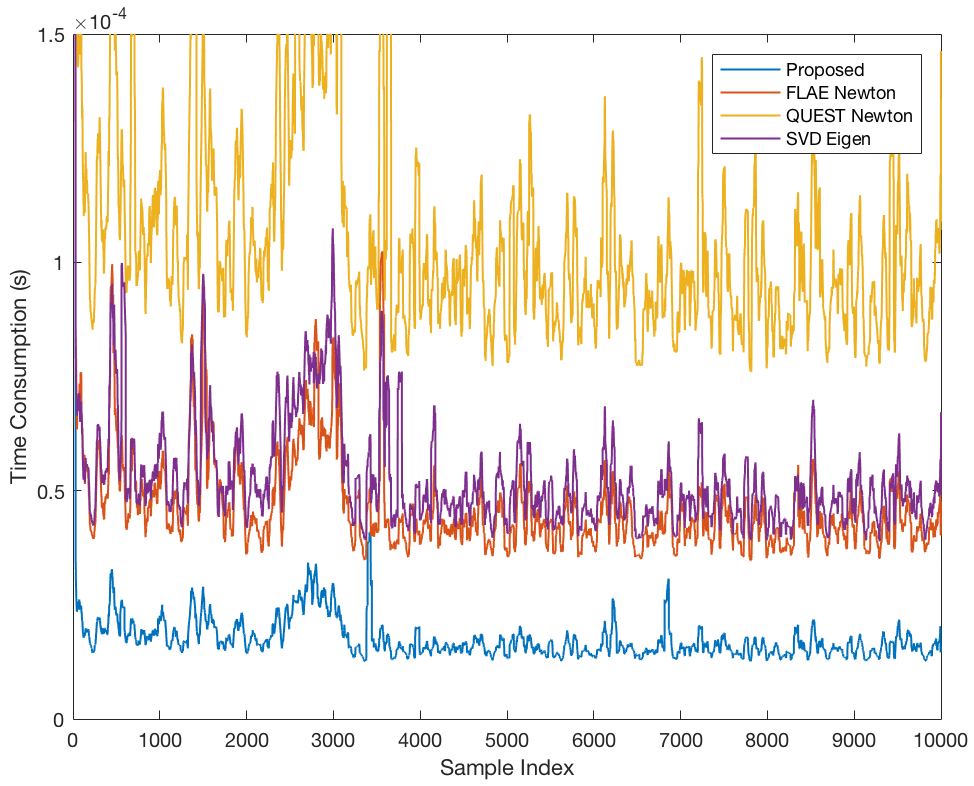
\includegraphics[width=1.0\textwidth]{time.jpg}
\caption{Execution time consumption of various algorithms.}
\label{fig:time}
\end{figure}

\section{Conclusion}
In this paper, we solve the problem of estimating the best rotation for the alignment of two sets of corresponding 3D vectors. It is based on solving the linear equations derived from the formulation of the problem in Geometric Algebra. The method is fast, robust to noise, accurate and simpler than most other methods. Experimental validation of the performance of the proposed algorithm is presented. The results show that the slightly losing accuracy of the proposed method is well worth the huge advance in execution time consumption. For many applications the vector datasets are very huge i.e. the computation time would be more important than slight change of accuracy. Therefore, we hope that the proposed algorithm would be of benefit to such applications.

\section{Acknowledgement}
This research is supported by National Natural Science Foundation  of China (NSFC) under the grant of No. 11701496.

\section{Conflict of Interests}
The authors declare no conflict of interests regarding the publication of this paper.

\section{C++ code}

\begin{lstlisting}[language=C++, caption=C++ code for rotor estimation, basicstyle=\tiny, keywordstyle=\bfseries, label=lst:cppcode, morekeywords={Matrix4d,Vector4d,Vector3d,Quaterniond,sqrt}]
Quaterniond FastRotorEstimator(
	vector<Vector3d>& P, vector<Vector3d>& Q, vector<double>& weights)
{
	Matrix4d H;
	Vector4d g, R, R_i;
	Vector3d S, D;
	const double epsilon = 1e-6;
	double wj;
	const size_t N = P.size();

	H.setZero();
	for (size_t j = 0; j < N; ++j) {
		wj = weights[j];
		S = Q[j] + P[j];
		D = P[j] - Q[j];
		H(0, 0) += wj*(D[0]*D[0] + D[1]*D[1] + D[2]*D[2]);
		H(0, 1) += wj*(D[0]*S[1] - D[1]*S[0]);
		H(0, 2) += wj*(D[0]*S[2] - D[2]*S[0]);
		H(0, 3) += wj*(D[1]*S[2] - D[2]*S[1]);
		H(1, 1) += wj*(S[1]*S[1] + S[0]*S[0] + D[2]*D[2]);
		H(1, 2) += wj*(S[1]*S[2] - D[2]*D[1]);
		H(1, 3) += wj*(D[2]*D[0] - S[0]*S[2]);
		H(2, 2) += wj*(S[2]*S[2] + S[0]*S[0] + D[1]*D[1]);
		H(2, 3) += wj*(S[0]*S[1] - D[1]*D[0]);
		H(3, 3) += wj*(S[2]*S[2] + S[1]*S[1] + D[0]*D[0]);
	}
	H(1, 0) = H(0, 1);
	H(2, 0) = H(0, 2); H(2, 1) = H(1, 2);
	H(3, 0) = H(0, 3); H(3, 1) = H(1, 3); H(3, 2) = H(2, 3);
	g = -H.col(0);
	H(0, 0) += epsilon; H(1, 1) += epsilon; 
	H(2, 2) += epsilon; H(3, 3) += epsilon;
	H = H.inverse();
	R(0) = 1; R(1) = 0; R(2) = 0; R(3) = 0;
	do {
		R_i = R;
		R(0) -= 1.0;
		R.noalias() = H * (g + epsilon * R);
		R(0) += 1.0;
		R /= sqrt(R.dot(R));
	} while ((R_i - R).dot(R_i - R) > 1e-6);
	return Quaterniond(R(0), -R(3), R(2), -R(1));
}
\end{lstlisting}

\bibliographystyle{abbrv}
\bibliography{rotorestimation}

% ------------------------------------------------------------------------
\end{document}
% ------------------------------------------------------------------------
